\documentclass{standalone}

\usepackage{tikz}
\usetikzlibrary{arrows.meta}
\usetikzlibrary{positioning}

\renewcommand{\familydefault}{\sfdefault}

\begin{document}

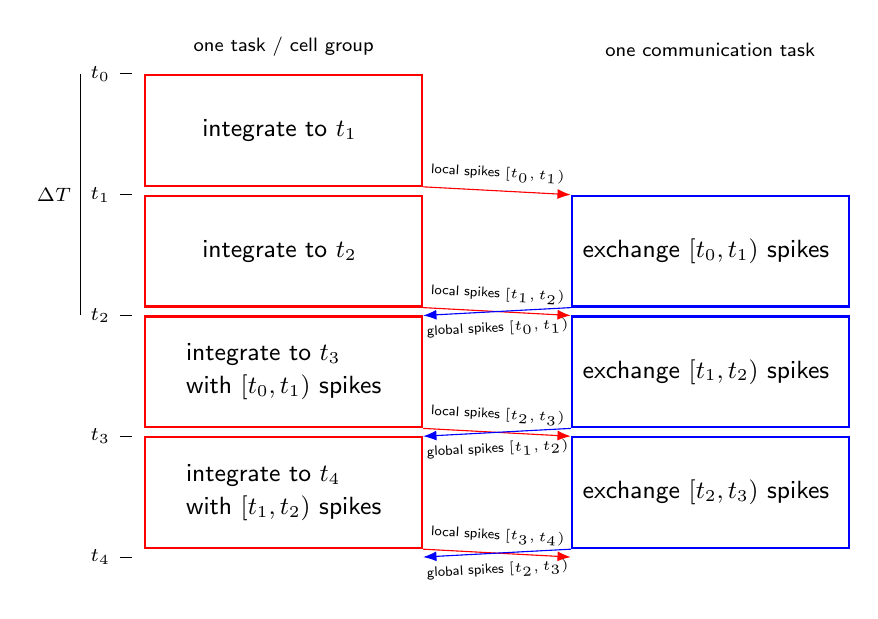
\begin{tikzpicture}
    [a/.style={rectangle, draw=red, thick, minimum height=9ex, minimum width=10em, align=left},
     b/.style={rectangle, draw=blue, thick, minimum height=9ex, minimum width=10em, align=left},
     ab/.style={-Latex, draw=red, fill=red},
     ba/.style={Latex-, draw=blue, fill=blue},
     tn/.style={minimum width=1em, align=left}]

    \node [a, align=left] (a0) {
	\small integrate to $t_1$
    };
    \node [a, below=1mm of a0, align=left] (a1)  {
	\small integrate to $t_2$
    };
    \node [a, below=1mm of a1] (a2) {
	\small integrate to $t_3$\\
	\small with $[t_0, t_1)$ spikes
    };
    \node [a, below=1mm of a2] (a3)  {
	\small integrate to $t_4$\\
	\small with $[t_1, t_2)$ spikes
    };
    \node [a, below=1mm of a3, minimum height=1ex, draw=none] (a4) {};

    \node [b, right=12ex of a0, draw=none] (b0) {};
    \node [b, right=12ex of a1] (b1) {
	\small exchange $[t_0,t_1)$ spikes
    };
    \node [b, right=12ex of a2] (b2) {
	\small exchange $[t_1,t_2)$ spikes
    };
    \node [b, right=12ex of a3] (b3) {
	\small exchange $[t_2,t_3)$ spikes
    };
    \node [b, right=12ex of a4, minimum height=1ex, draw=none] (b4) {};

    \draw [ab] (a0.south east) -- node [sloped, above] {\tiny local spikes $[t_0, t_1)$} (b1.north west);
    \draw [ab] (a1.south east) -- node [sloped, above] {\tiny local spikes $[t_1, t_2)$} (b2.north west);
    \draw [ab] (a2.south east) -- node [sloped, above] {\tiny local spikes $[t_2, t_3)$} (b3.north west);
    \draw [ab] (a3.south east) -- node [sloped, above] {\tiny local spikes $[t_3, t_4)$} (b4.north west);

    \draw [ba] (a2.north east) -- node [sloped, below] {\tiny global spikes $[t_0, t_1)$} (b1.south west);
    \draw [ba] (a3.north east) -- node [sloped, below] {\tiny global spikes $[t_1, t_2)$} (b2.south west);
    \draw [ba] (a4.north east) -- node [sloped, below] {\tiny global spikes $[t_2, t_3)$} (b3.south west);

    \draw ([xshift=-1ex] a0.north west) -- ++(-1ex, 0) node [tn, left] (t0) {\scriptsize $t_0$};
    \draw ([xshift=-1ex] a1.north west) -- ++(-1ex, 0) node [tn, left] {\scriptsize $t_1$};
    \draw ([xshift=-1ex] a2.north west) -- ++(-1ex, 0) node [tn, left] (t2) {\scriptsize $t_2$};
    \draw ([xshift=-1ex] a3.north west) -- ++(-1ex, 0) node [tn, left] {\scriptsize $t_3$};
    \draw ([xshift=-1ex] a4.north west) -- ++(-1ex, 0) node [tn, left] {\scriptsize $t_4$};

    \draw (t0.west) -- node [left] {\scriptsize $\Delta T$} (t2.west);

    \node [above=1mm of a0.north] {\scriptsize one task / cell group};
    \node [above=1mm of b0.north] {\scriptsize one communication task};
\end{tikzpicture}

\end{document}
